\documentclass[12pt]{article}
\usepackage[english]{babel}
\usepackage{subcaption}
\usepackage{float}
\usepackage{natbib}
\usepackage{url}
\usepackage[utf8x]{inputenc}
\usepackage{amsmath}
\usepackage{graphicx}
\graphicspath{{images/}}
\usepackage{parskip}
\usepackage{fancyhdr}
\usepackage{vmargin}
\usepackage{listings}
\usepackage{color} %red, green, blue, yellow, cyan, magenta, black, white
\definecolor{mygreen}{RGB}{28,172,0} % color values Red, Green, Blue
\definecolor{mylilas}{RGB}{170,55,241}


\setmarginsrb{3 cm}{2.5 cm}{3 cm}{2.5 cm}{1 cm}{1.5 cm}{1 cm}{1.5 cm}
\usepackage{listings}
\title{Spot Welding Robot}
\author{Akwasi A. Obeng}                    
\date{December 08, 2019}										
\makeatletter
\let\thetitle\@title
\let\theauthor\@author
\let\thedate\@date
\makeatother

\pagestyle{fancy}
\fancyhf{}
\rhead{\theauthor}
\lhead{\thetitle}
\cfoot{\thepage}

\begin{document}

%%%%%%%%%%%%%%%%%%%%%%%%%%%%%%%%%%%%%%%%%%%%%%%%%%%%%%%%%%%%%%%%%%%%%%%%%%%%%%%%%%%%%%%%%

\lstset{language=Matlab,%
    %basicstyle=\color{red},
    breaklines=true,%
    morekeywords={matlab2tikz},
    keywordstyle=\color{blue},%
    morekeywords=[2]{1}, keywordstyle=[2]{\color{black}},
    identifierstyle=\color{black},%
    stringstyle=\color{mylilas},
    commentstyle=\color{mygreen},%
    showstringspaces=false,%without this there will be a symbol in the places where there is a space
    numbers=left,%
    numberstyle={\tiny \color{black}},% size of the numbers
    numbersep=9pt, % this defines how far the numbers are from the text
    emph=[1]{for,end,break},emphstyle=[1]\color{red}, %some words to emphasise
    %emph=[2]{word1,word2}, emphstyle=[2]{style},    
  }


\begin{titlepage}
	\centering
    \vspace*{0.5 cm}
    
\includegraphics[scale = 0.1]{uon.jpeg}\\[1.0 cm]	% University Logo
    \textsc{\LARGE ENPM662(Robot Modelling)}\\[2.0 cm]	% University Name
	\textsc{\Large Formal Report}\\[0.5 cm]				% Course Code
	\textsc{\large Project}\\[0.5 cm]				% Course Name
	\rule{\linewidth}{0.2 mm} \\[0.4 cm]
	{ \huge \bfseries \thetitle}\\
	\rule{\linewidth}{0.2 mm} \\[1.5 cm]
	
	\begin{minipage}{0.4\textwidth}
		\begin{flushleft} \large
			\emph{Author:}\\
			\theauthor
			\end{flushleft}
			\end{minipage}~
			\begin{minipage}{0.4\textwidth}
			\begin{flushright} \large
			\emph{UID:} \\
			117000801									% Your Student Number
		\end{flushright}
	\end{minipage}\\[2 cm]
	
	{\large \thedate}\\[2 cm]
 
	\vfill
	
\end{titlepage}

%%%%%%%%%%%%%%%%%%%%%%%%%%%%%%%%%%%%%%%%%%%%%%%%%%%%%%%%%%%%%%%%%%%%%%%%%%%%%%%%%%%%%%%%%

\tableofcontents
\pagebreak

%%%%%%%%%%%%%%%%%%%%%%%%%%%%%%%%%%%%%%%%%%%%%%%%%%%%%%%%%%%%%%%%%%%%%%%%%%%%%%%%%%%%%%%%%

\section{Motivation}
\paragraph{}
Automated Welding is a practical necessity in companies today as it is much safer, cheaper and more robust. Different companies
from Automobile to Delivery make of use welding robots and this has resulted in a boost in 
productivity.The surge in 
the development of welding robots not only lies in the safety it offers but rather in the precision and accuracy with which it is achieved.In the automation industry,
welding robots are used for a variety 
of tasks, from resistance welding (join metal surfaces together
through the application 
heat by resistance of electric current) to arc welding. Refer to \url{https://en.wikipedia.org/wiki/Arc_welding} for 
more information. The type of welding to be looked at is \textbf{Spot welding} and is a type of resistance welding which 
involves joining two thin metals that resist electric currents.

\begin{figure}[H],
    \centering
    %\textbf{your title}\par\medskip
    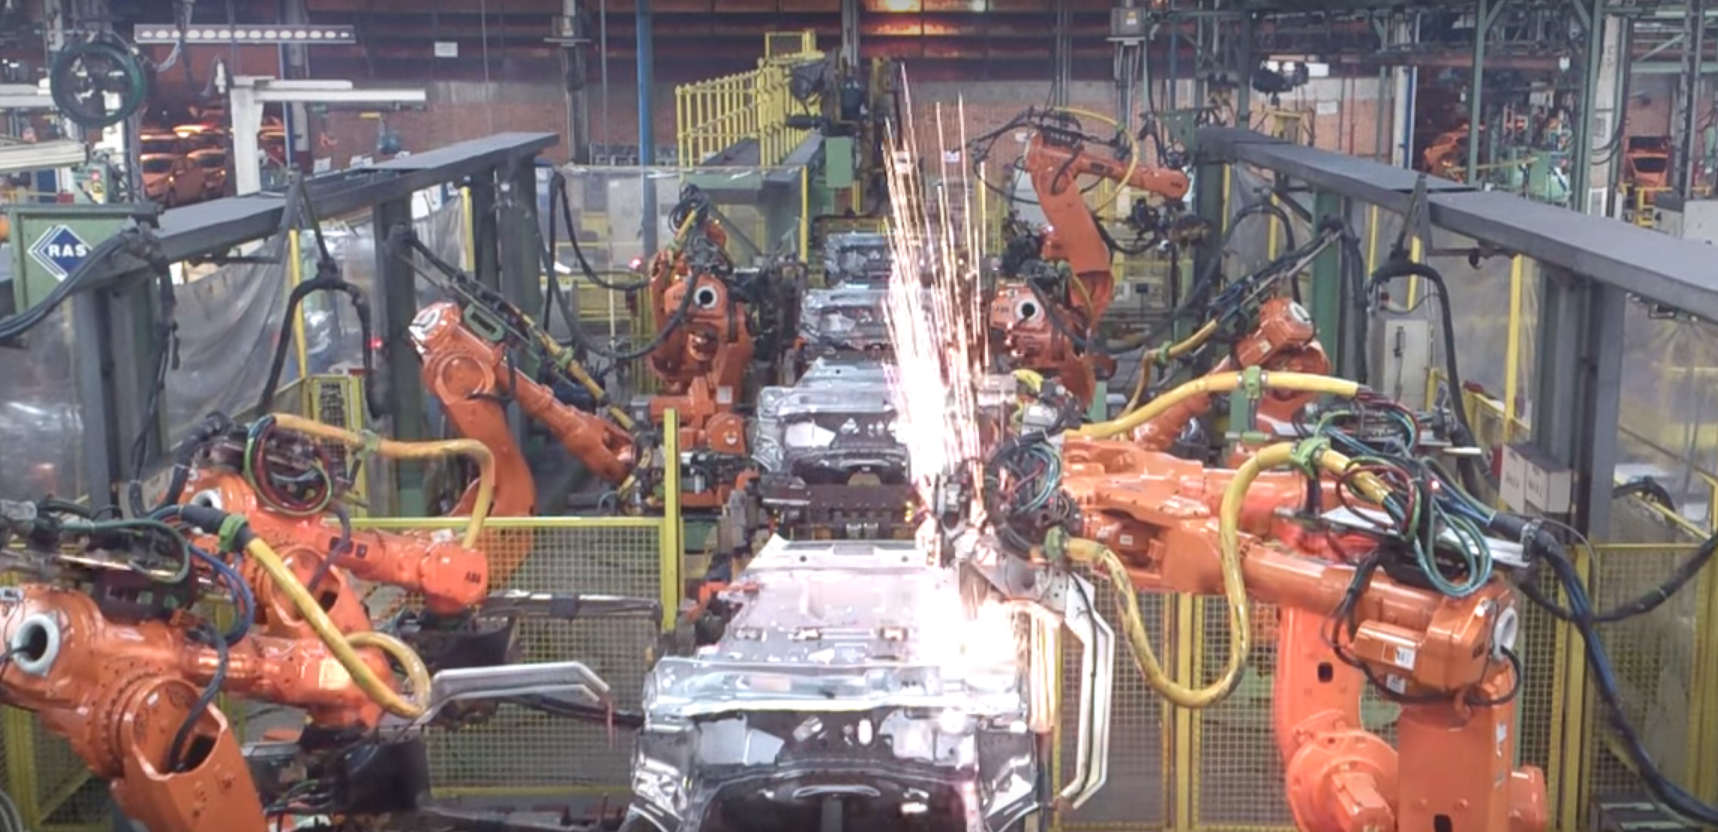
\includegraphics[scale = 0.2]{welding.png}\\[0.0 cm]	% University Logo
    \caption{Welding in Automotive industry} 
\end{figure}

\paragraph{}
Welding Robots are designed to perform a specific 
task and in other for this to be achieved, the 
control system, sensing system and the 
different components of the robot must 
function well to 
achieve some desired result. Precision is of the essence as the robot is supposed to join(weld) two spots together  at the 
some \textbf{specified location}, with the right \textbf{amount of force} whilst operating at some \textbf{optimum speed} for productivity.Should the robot
be off in its measurement by even a few centimeters,then this could be detrimental to the whole operation. \textbf{Precision is of paramount importance}.This project looks at how this can be achieved.



\section{Introduction}
\paragraph{}
The focus of this project is on how a welding robot can be modelled with precision to achieve some desired task.
The robot to be simulated should in principle be able to join metal plates together. 
For brevity, a specialized robotic arm (robotic arm modified to meet required task) is used.
That is given some metal plates, the robot should efficiently navigate its environment,
handle appropriate weights and operate within some required standards.

The robot to be simulated must satisfy the following criteria
\begin{itemize}
   \item Have a good workspace range
   \item Have tapering ends for piercing metal sheets
   \item Must be able to position itself to weld some specified locations
\end{itemize}

\section{Model Design}
 Based on the requirements, the design below was created
\begin{figure}[H],
    \centering
    %\textbf{your title}\par\medskip
    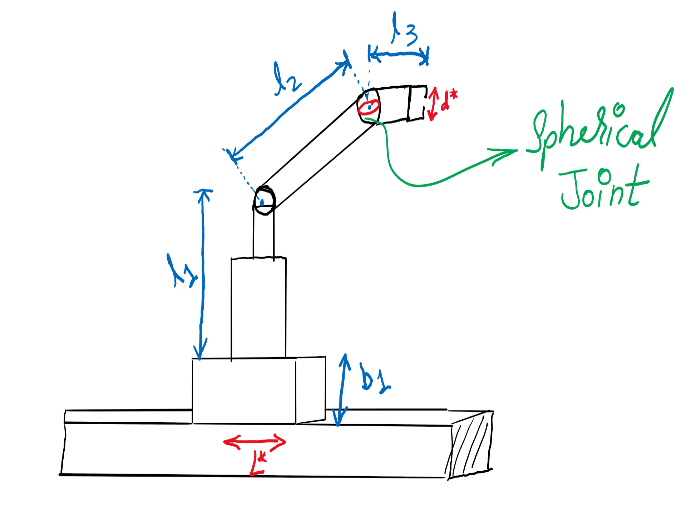
\includegraphics[scale = 1.1]{design.png}\\[0.0 cm]	% University Logo
    \caption{Robot Design} 
\end{figure}
\textbf{Robot Attributes}
\begin{itemize}
  \item 6 Degrees of Freedom(DOF) not including the end effector 
  \item 1 prismatic joint(Rack and pinion) at the base and 5 revolute joints 
  \item Link lengths $l1>l2>l3$
  \item End effector has tapering ends for piercing effect 
\end{itemize}

\begin{figure}[H]
    \centering
    %\textbf{your title}\par\medskip
    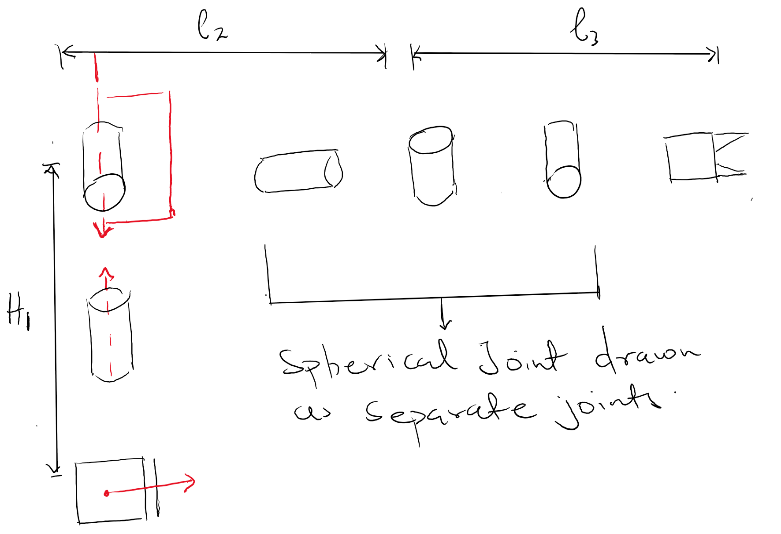
\includegraphics[scale = 1.1]{joints.png}\\[0.0 cm]	% University Logo
    \caption{Joints of Robot} 
\end{figure}
 \subsection{workspace}
 Due to the complexity of the workspace, the projected workpace is used.
 \begin{figure}[H]
    \centering
    %\textbf{your title}\par\medskip
    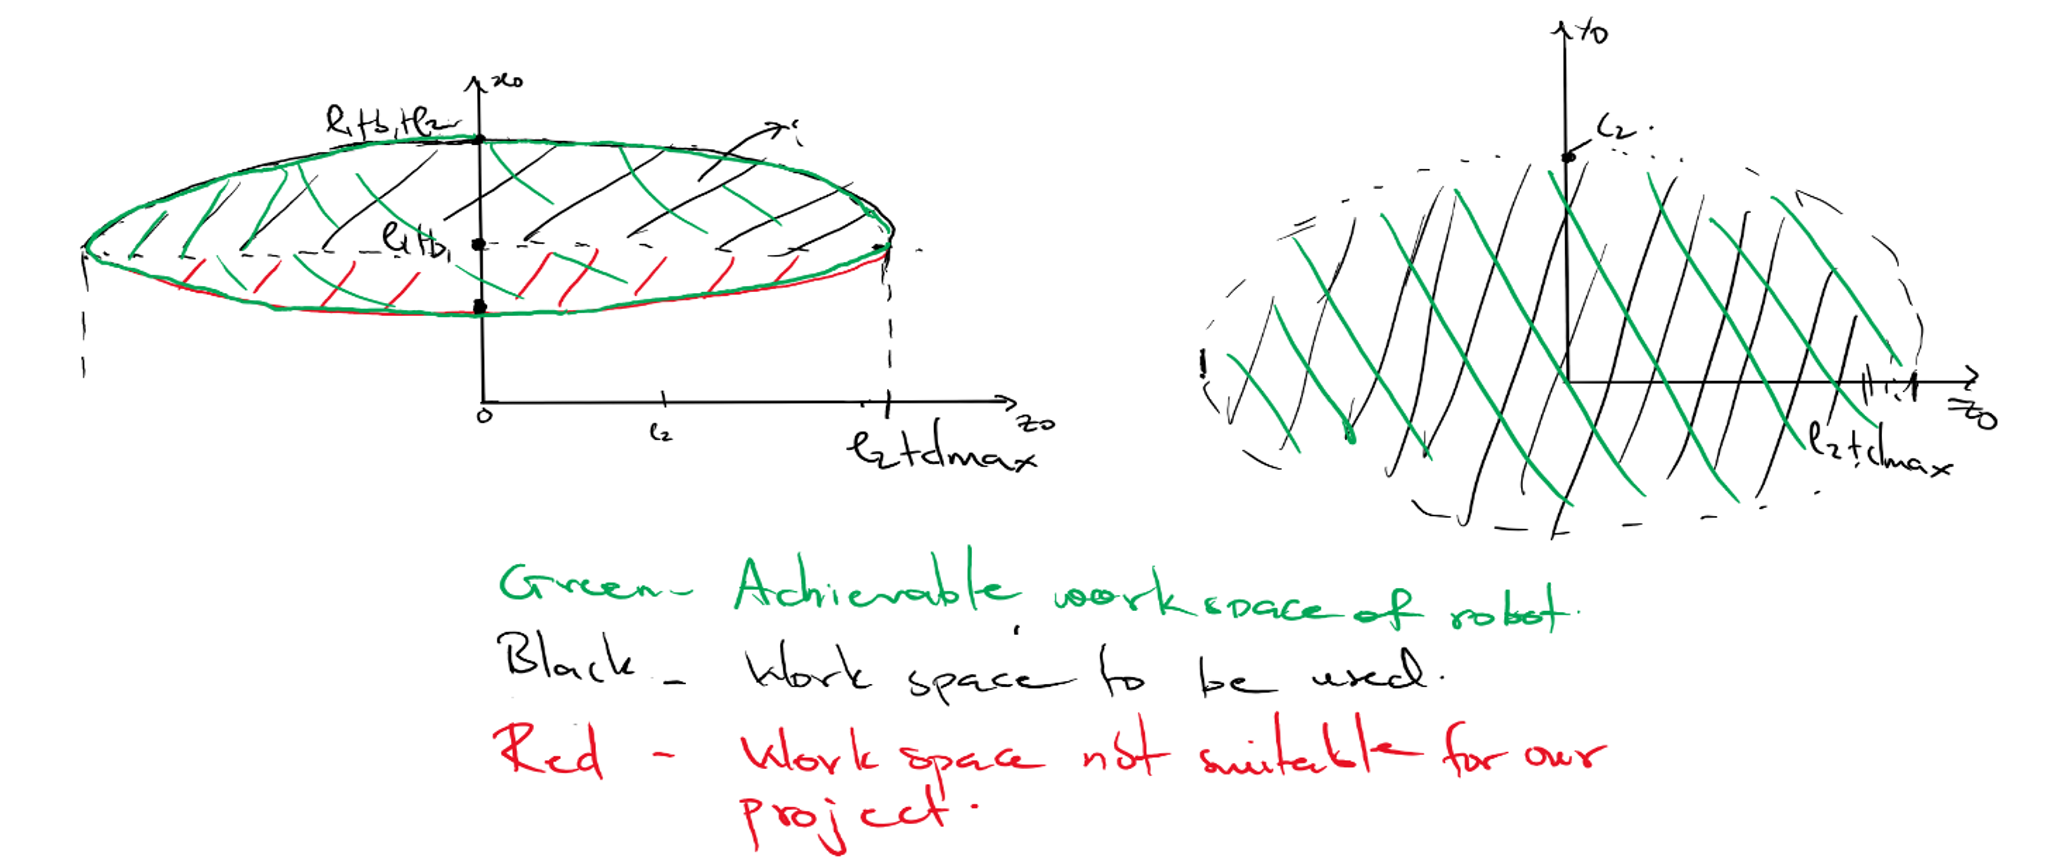
\includegraphics[scale = 0.65]{workspace.PNG}\\[0.0 cm]	% University Logo
    \caption{Workspace}
 \end{figure}


 \section{Kinematics}
In this section, the forward and inverse kinematics calculations are  performed for the robot described above.
\subsection{Foward Kinematics}
\begin{figure}[H]
    \centering
    %\textbf{your title}\par\medskip
    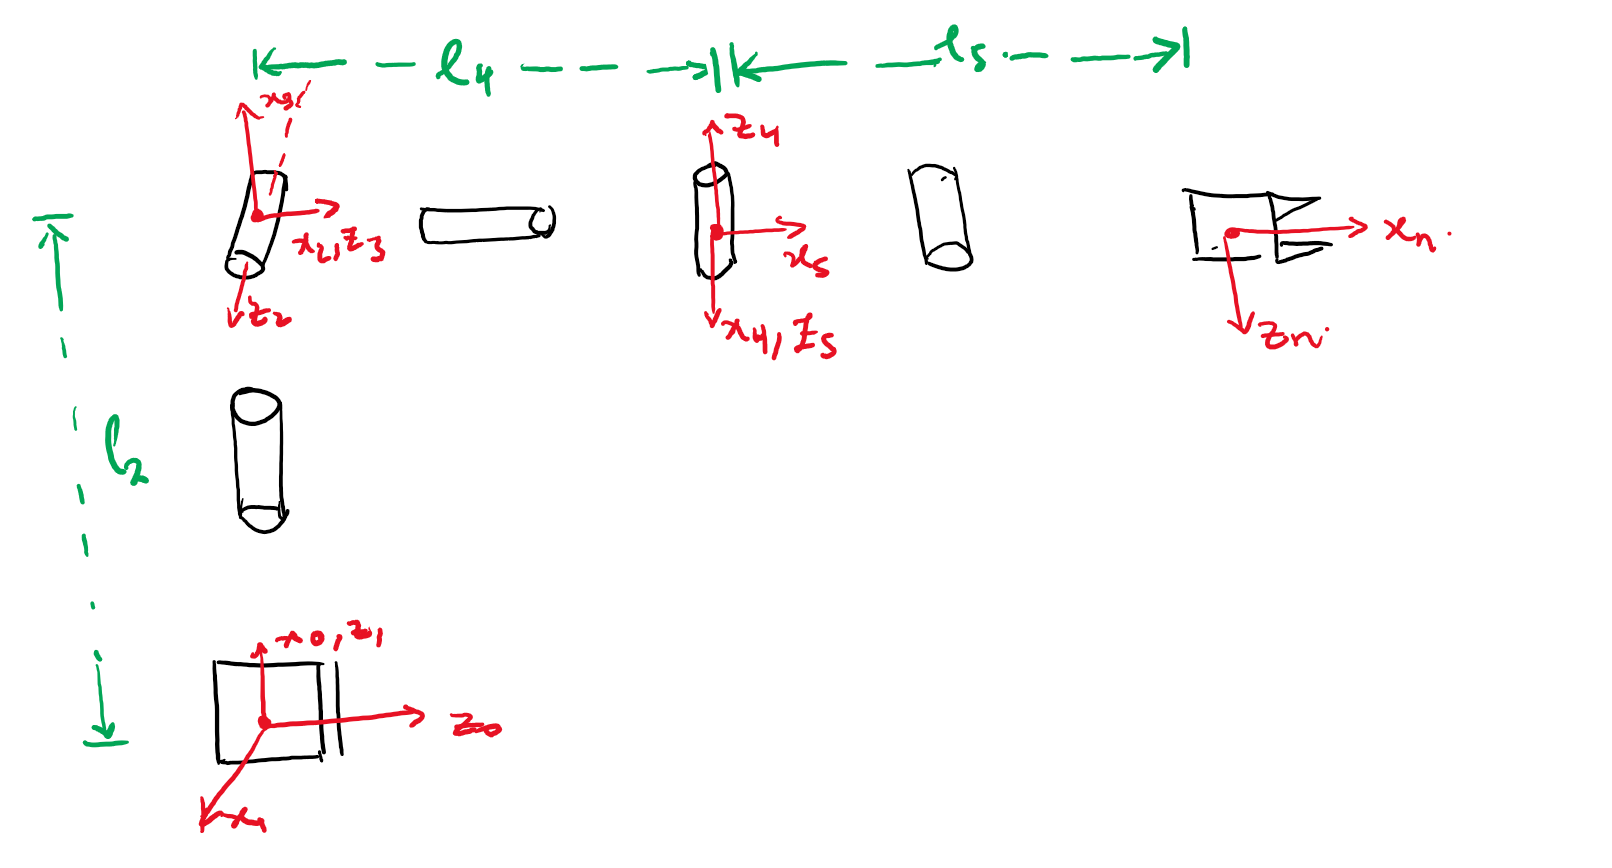
\includegraphics[scale = 0.7]{forward.png}\\[0.0 cm]	% University Logo
    \caption{Assigning DH Frames}
\end{figure}


\begin{tabular}{ |p{3cm}||p{3cm}|p{3cm}|p{3cm}|p{3cm}| }
 \hline
 \multicolumn{5}{|c|}{DH Table} \\
 \hline
 T&$\theta$&d&a&$\alpha$\\
 \hline
 $0->1$ & $90^0$    &$d_1^*$ & 0 &$90^0$  \\
 $1->2$ & $\theta _1^*+90^0$    &$l_2$$ & 0 &$90^0$  \\
 $2->3$ & $\theta _2^*+90^0$    &0 & 0 &$90^0$  \\
 $3->4$ & $\theta _3^*+90^0$    &$l_4$ & 0 &$90^0$  \\
 $4->5$ & $\theta _3^*+90^0$   &0 & 0 &$90^0$  \\
 $5->n$ & 0    &0 & $l_5$ &$0$ \\
 \hline
\end{tabular}
\\ \\ \\
\textbf{DH calculations}

The DH table is represented as follows \\
\resizebox{0.8\textheight}{0.08\textwidth}{  
  T_0^n =
\begin{bmatrix}
    c_4s_2+c_2s_3s_4 & c_2c_3 & s_2s_4-c_2c_4s_3 & l_2+l_5(c_4s_2+c_2s_3s_4)+l_4s_2 \\
    -s_4c_1c_3-s_1s_2s_3-c_2c_4s_1 & c_1s_3+c_3s_1s_2 &c_4(c_1c_3-s_1s_2s_3)-c_2s_1s_4 & -l_5(s_4(c_1c_3-s_1s_2s_3)+ c_2c_4s_1)-l_4c_2s_1 \\
    c_1c_2c_4-s_4(c_3s_1+c_1s_2s_3) &s_1s_3-c_1c_3s_2 & c_4(c_3s_1+c_1s_2s_3)+c_1c_2s_4&d_1-l_5(s_4(c_3s_1+c_1s_2s_3)-c_1c_2c_4)+l_4c_1c_2 \\
    0 & 0 &0 & 1
\end{bmatrix}
} 

\paragraph{}\textbf{Refer to the Appendix(Code for DH Table)} for the code used in generating the dh table.

\subsection{Inverse Kinematics}
Since robot has six degree freedom and a spherical wrist, the problem is decoupled into 
two parts, that is 
\begin{itemize}
  \item Finding Wrist center
  \item Orientation of Wrist
\end{itemize}

\paragraph{}
\textbf{Finding Wrist Center}
Suppose the wrist center is located at the coordinates $X_c, Y_c, Z_c$ the required joint angle 
parameters are obtained as follows
\begin{figure}[H]
  \begin{subfigure}{.5\textwidth}
    \centering
    \textbf{Top View}\par\medskip
    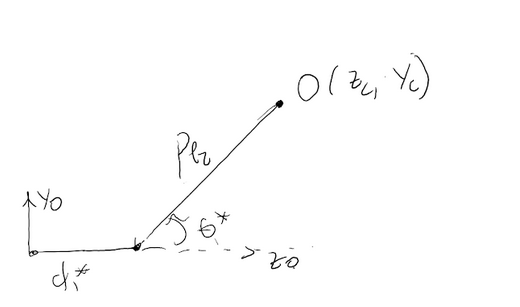
\includegraphics[scale = 0.5]{topview.png}\\[0.0 cm]	% University Logo
    \caption{Inverse kinematics}
     
\begin{align}
  \theta_2^* &= \sin ^{-1}(\frac{Y_c}{Pl_2}) \\
  d_1^* &= Z_c -Pl_2cos(\theta_1^*) 
\end{align}
  \end{subfigure}
\begin{subfigure}{.5\textwidth}
    \centering
    \textbf{Side View}\par\medskip
    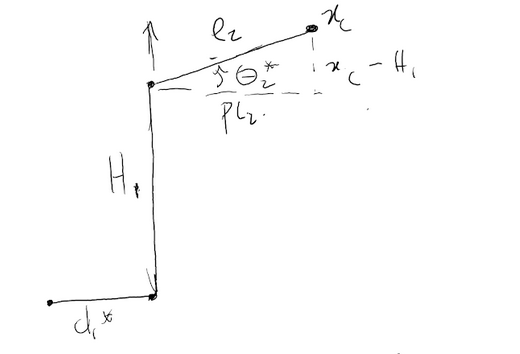
\includegraphics[scale = 0.5]{sideview.png}\\[0.0 cm]	% University Logo
    \caption{Inverse kinematics}
\begin{align}
  \theta_3^* &= \sin ^{-1}(\frac{X_c - H}{l_2})  \\
Pl_2 &= l_2cos(\theta_3^*h)
\end{align}
\end{subfigure}
\end{figure}
Therefore,
\begin{align}
  \theta_2^* &= sin^{-1}(\frac{Y_c}{Pl_2}) \\
  \theta_3^* &= \sin ^{-1}(\frac{X_c - H}{l_2})  \\
  d_1^* &= Z_c -l_2*cos(h(\sin ^{-1}(\frac{X_c - H}{l_2})))cos(sin^{-1}(\frac{Y_c}{Pl_2}))
\end{align}\\ 

The values of $X_c,Y_c$ and $Z_c$ can be gotten from $O_4$(Refer to Appendix(Code for Jacobian)).
\\
\textbf{NB Since there is a prismatic joint at the base, it is possible to get 2 or \\
more solutions for the wrist center}. To visualize this consider the case shown below

\begin{figure}[H]
    \centering
    \textbf{Multiple Solutions}\par\medskip
    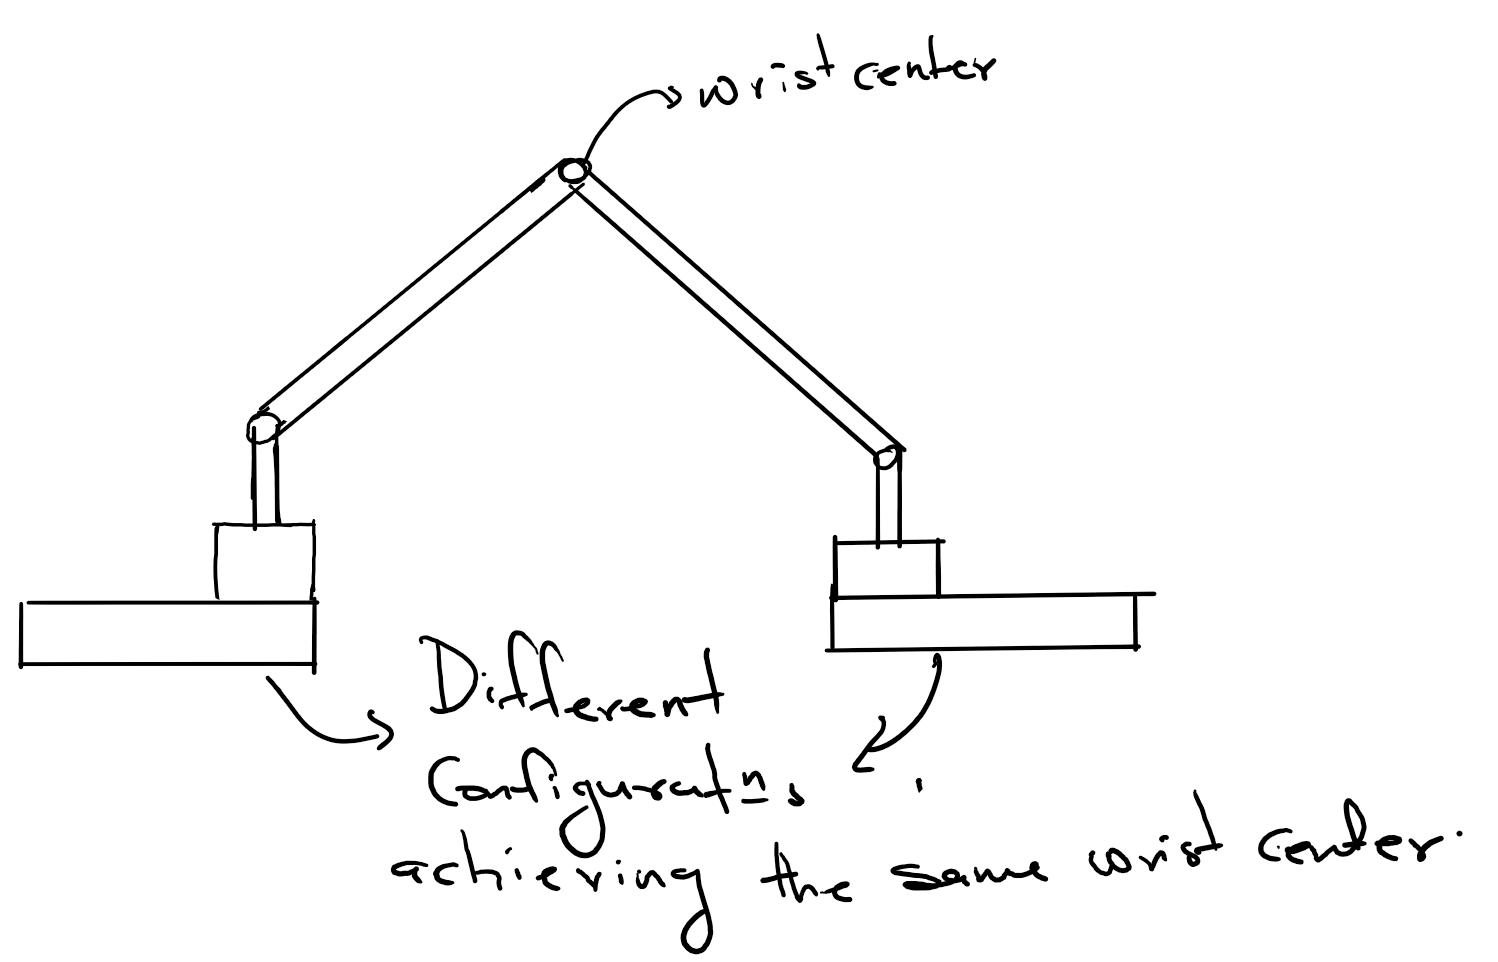
\includegraphics[scale = 0.5]{multisol.png}\\[0.0 cm]	% University Logo
  \end{figure}
\paragraph{}

\textbf{Orientation of Wrist} \\
The actual calculations needed to get the angles for orienting the sperical wrist is not provided but rather a cursory overview on how this can be achieved.
The orientation of the wrist can be gotten as follows
\begin{align}
  R^0_6 &= R^0_3R^3_6 \\
  R^3_6 &= R^3_0R^0_6
\end{align}
$R^3_0$ is known  from previous calcuations and $R^0_6$ is known from the DH table. \\ \\
Representing $R^3_6$ as a zyz transformation, the following angles $\theta,\phi, \gamma$ can be obtained
by comparing matrix with the product of $R^3_0R^0_6$ and solving for the angles.  \\ \\

\textbf{NB. Infinite number of solutions when the robot is in an upright position}
\section{Piercing, and Singularity}
The amount of force needed at the endeffector(gripper)  to pierce the metal sheet is material dependent.
Therefore, only the general form of the wrench is obtained.

\begin{equation}
   T = J^T(q)F
\end{equation}
where T is the  joint torque,F is the endeffector wrench and J is the jacobian.
Refer to \textbf{Appendix(Code for Jacobian)} for  calculation of Jacobian \\ \\
\textbf{Singularity} \\
Since the robot has a spherical joint, it has a singularity(wrist flip) when the robot is in an upright(projected) position.
To get all the values of q for which the Jacobian has a singular configuration,
we find   
\begin{equation}
  Det(J) = 0
\end{equation}
The calculation of the determinant of J is quite cumbersome since J is a 6x6 matrix.
The calculation can be decoupled into two components, ie 
\begin{align}
  Det(J_{3:6}^{1:3}) =0 \\
  Det(J_{1:3}^{3:6}) =0
\end{align}
That is the determinant of the upper right and lower left blocks of the jacobian can be calculated and the values of q for which
a singularity occurs can then be obtained. 
However, for the purporse of this project, all the possible values for which a singular configuration occurs is not of interest.
We only need to check if there is some singularity along some predetermined path and this can be done by careful inspection.


\section{Simulation}
 For convenience of simulation, the original design is modified to yield
 the figure shown below.
 \begin{figure}[H]
    \centering
    \textbf{Modified Design}\par\medskip
    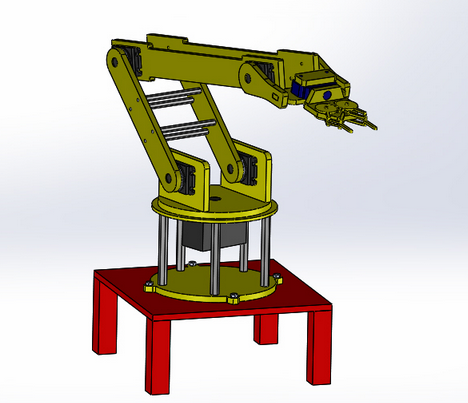
\includegraphics[scale = 0.4]{newmodel.png}\\[0.0 cm]	% University Logo
    \caption{CAD Model}
\end{figure} 
Clearly the new model above differs from the original design. However, this new model can be considered as a restricted version of the old design. Futher emphasis is provided in the next section.
  
  \subsection{Constraints and Design Modifications}
  \begin{itemize}
    \item \textbf{Modified base} \\
    Instead of a movable base, a fixed base is used in the simulation.
  \begin{figure}[H]
    \centering
    \textbf{Changing Base}\par\medskip
    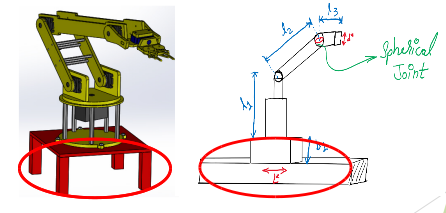
\includegraphics[scale = 0.67]{modifiedbase.png}\\[0.0 cm]	% University Logo
    \caption{Modified Base}
  \end{figure} 
  This can however be viewed as the original design constrained to some fixed location.
  That  is 
  \begin{equation}
    d_1^*= constant(c) \quad  -\quad \text{\texbf{Holonomic Constraint}}
  \end{equation} \\ 

  \item \textbf{Modified Spherical Joint} \\
     Instead of a spherical joint at the wrist, only 2 revolute joints are used
  \begin{figure}[H]
    \centering
    \textbf{Changing Spherical joint}\par\medskip
    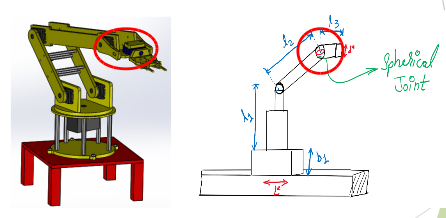
\includegraphics[scale = 0.7]{modifiedjoint.png}\\[0.0 cm]	% University Logo
    \caption{Modified Spherical joint}
  \end{figure} 
  This can be viewed as the original design with the constraint as follows
  
  \begin{equation}
    \theta _5^* = constant(c) \quad  -\quad \text{\texbf{Holonomic Constraint}}
  \end{equation} \\ 

  \item \textbf{Increase Workspace Range} \\
    To increase workspace range, of the robot, one additional link and revolute joint is added 
   \begin{figure}[H]
    \centering
    \textbf{Changing Spherical joint}\par\medskip
    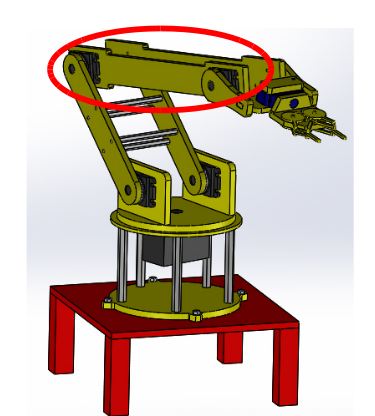
\includegraphics[scale = 0.4]{link.png}\\[0.0 cm]	% University Logo
    \caption{Added link and revolute joint}
   \end{figure} 
  \end{itemize}

  \item \textbf{Changing Endeffector}  \\
    For ease of simulation, an inbuilt Baxter gripper is used.
    
  \subsection{Assumptions}
  The following assumptions were made for simulation
  \begin{itemize}
    \item Singularity - The robot is never in a singular configuration. 
    \item Dynamical Forces  -Friction  and other dynamical forces associated with the moving object are not accounted for 
    \item Structure- The robot will operate within some structured environment.Objects(metal sheets) to be welded together
      are placed on a \textbf{conveyor belt} moving at a \textbf{constant speed}. The conveyor belt is equipped with sensors 
      to determine when an object is present and enough time is given to the robot to weld metal plates together.
    \item Conveyor belt does not accelerate when already in motion 
    \item There is enough gap between adjacent metal sheets been transported
    \item Metal sheet placed on conveyor belt is within reacheable workspace of robot
  \end{itemize}

  \subsection{Scope of Simulation}
  \begin{itemize}
    \item Forward and Inverse kinematics -  This was accounted for in the simulation
    \item Contact and Piercing- This was partially accounted for in the simulation. The baxter gripper used 
     does not have a piercing end and so although the calculations were made, the simulation didn't include this effect 
   \item Dynamics - Not Simulated. The (Inverse/Forward) mode was used in vrep and not the (torque/dynamics) mode.
   \item Constraints - This is accounted for by the modified model used in the simulation
  \end{itemize}
  
  \section{Vrep Scene}
   Components used for scene in Vrep.
   \textbf{Refer to Appendix(Simulation Components for Vrep)} for the full scene and code.
   \begin{itemize}
     \item Robot - The robot utilized is the cad Model(welding robot) that was descibed above.  
     \item Conveyor Belt - This is used to transport the objects(metal sheets) to be welded  together
     \item Sensors - These are used to indicate whether an object(metal sheet to be welded) is present
                     and also to determine whether the object has reached the end of the the conveyor belt.
     \item Metal Sheet - Metal sheets are depicted as a plane sandwiched between two blocks.
   \end{itemize}
   \begin{figure}[H]
    \centering
    \textbf{Simulation Enviroment}\par\medskip
    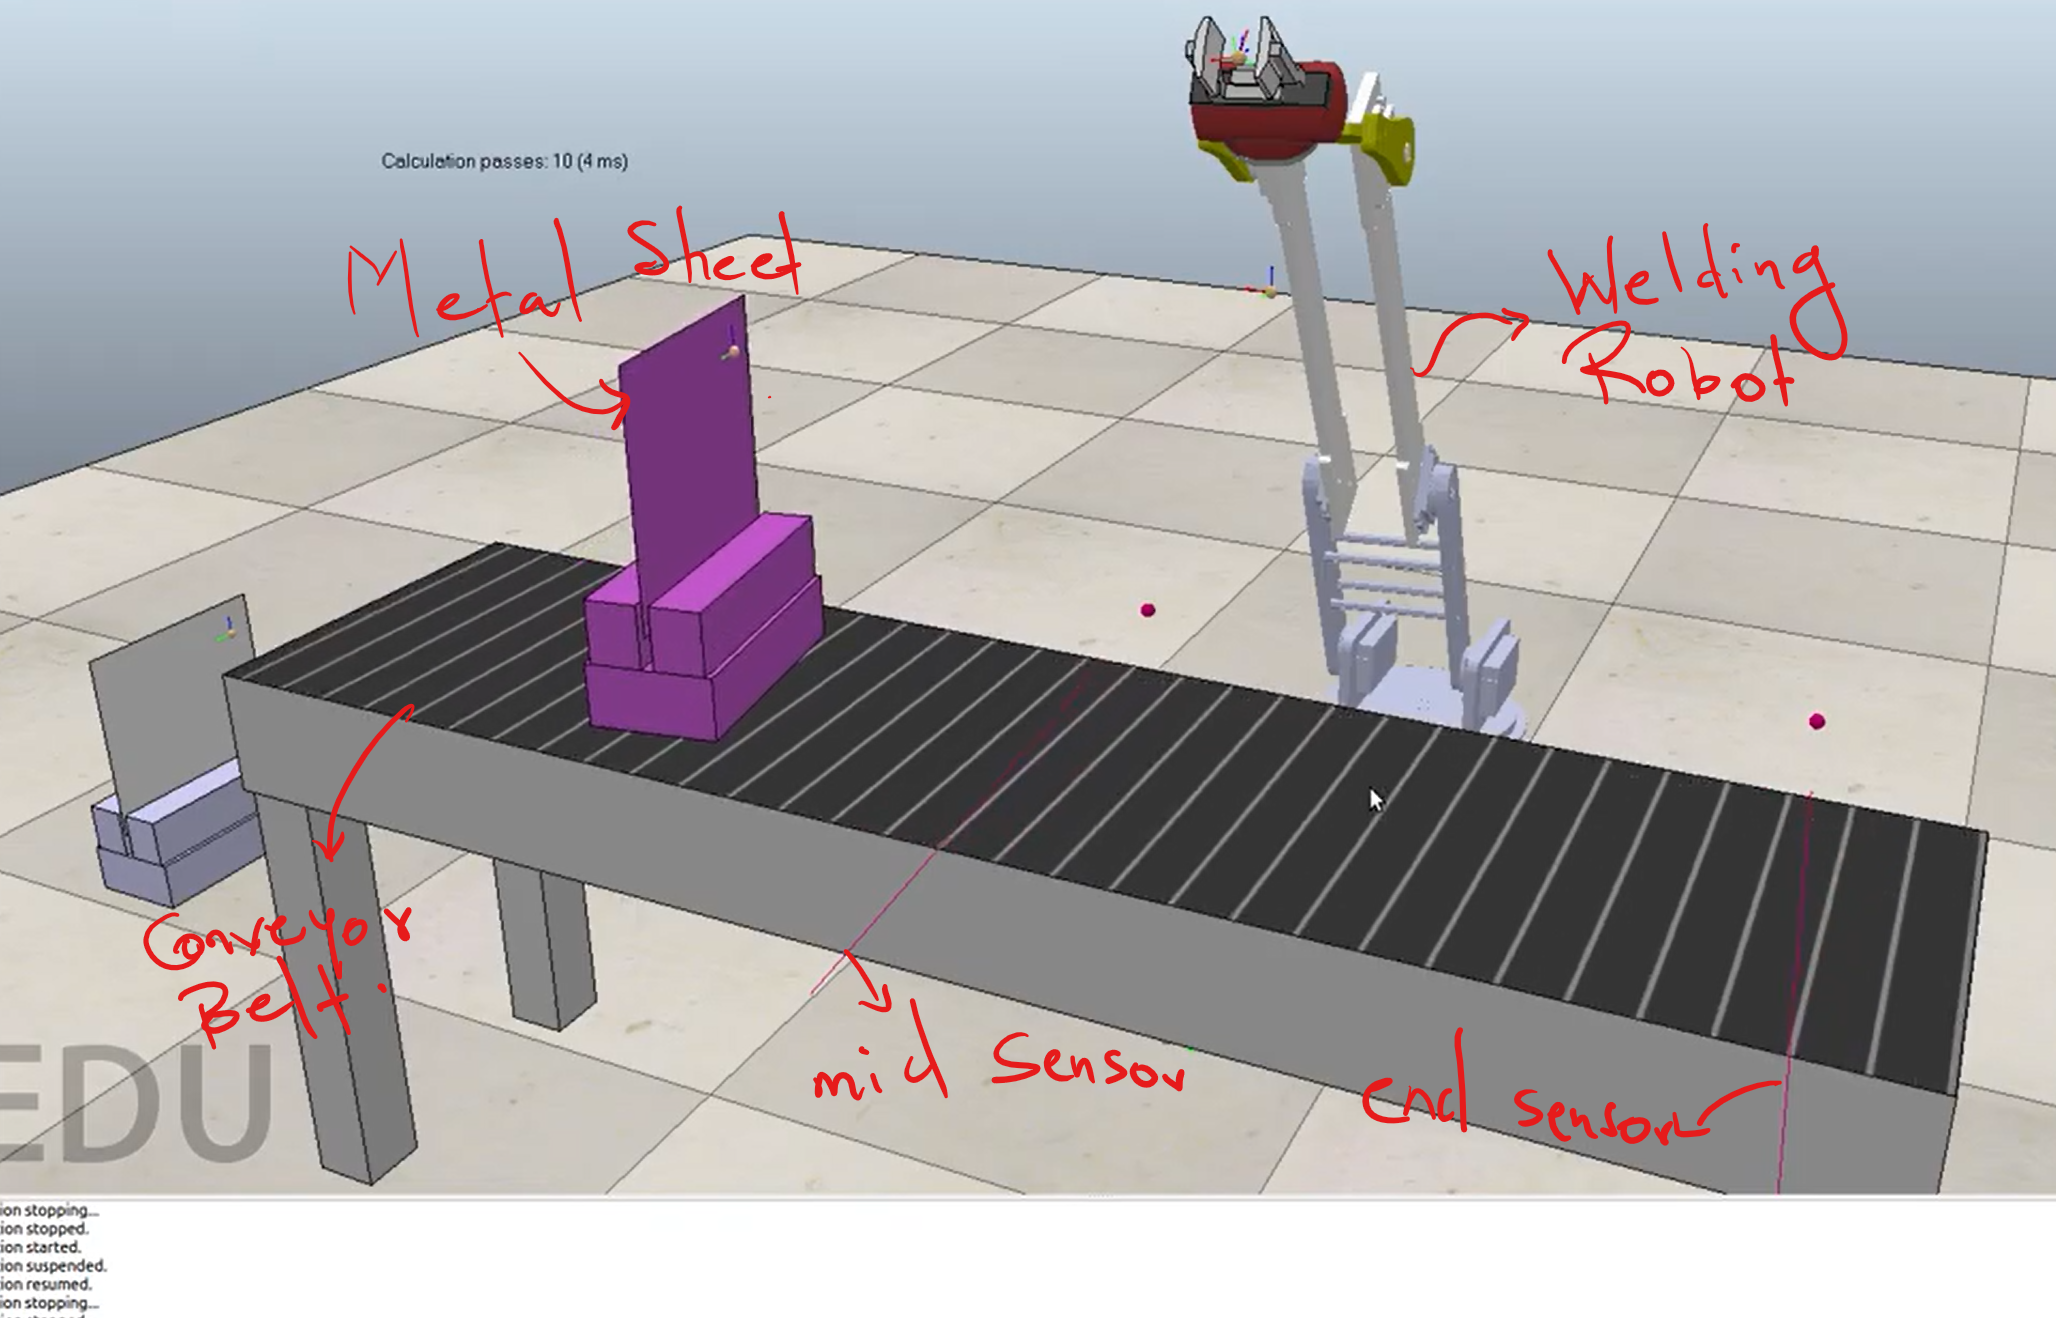
\includegraphics[scale = 0.5]{simenv.png}\\[0.0 cm]	% University Logo
    \caption{Components displayed in Simulation Environment}
   \end{figure} 
  \subsection{How the Code Works} \\
  A brief overview on how the code works is given below. 
  
  The code can be broken down into two key components 

  \textbf{Conveyor Belt}  -- Non Threaded
    \begin{enumerate}
        \item Continue to transport object on the conveyor belt
        \item If an item is sensed by mid sensor(Sensor located at the middle of the conveyor belt)
          \begin{enumerate}
             \item Stop Conveyor belt
             \item Wait for object to be processed(metal sheet to be welded)
             \begin{enumerate}
               \item If item has been processed, start the conveyor and continue transporting objects
             \end{enumerate}
          \end{enumerate}
        \item If an item is sensed at the end sensor(Sensor located at the end of the convyeor belt)
          \begin{enumerate}
            \item Delete Object
          \end{enumerate}
    \end{enumerate}

  \textbf{Welding Robot} --  Threaded
    \begin{enumerate} 
        \item Wait for an object to be sensed by the sensor in the middle of the conveyor belt 
          \begin{enumerate}
            \item If an object is sensed, follow a pickup path(path to object) 
            \item Weld the object(metal sheet)
            \item Send a signal to indicate object has been welded
            \item Follow a release path(path to return the object to its initial position) 
            \item Send a signal to indicate that it is okay for the conveyor belt to resume  transporting objects
            \item Wait for an object to detected again and repeat the process
          \end{enumerate}
    \end{enumerate}

\section{Testing and Validation}
  Visit the following url to view the simulation \\
  \url{https://www.youtube.com/watch?v=xeCUFldfl0U&feature=youtu.be} \\
  \url{https://www.youtube.com/watch?v=jMd6bSmziDo&feature=youtu.be} \\ \\
  \textbf{Testing Code and Parameters Used in simulation} \\
  Based on the simulation videos, it can be seen that the welding robot is able to position itself
  in a suitable orientation for welding metal sheets even when the metal sheet is slightly tilted.
  However, the piercing effect of the gripper is not properly done and this is partly due to the fact that the
  baxter gripper is not appropriate for application at hand. \\ \\
  
  \textbf{Forward and Inverse Verification} \\
Forward Kinematics
\begin{figure}[H]
  \begin{subfigure}{.5\textwidth}
    \centering
    \textbf{Base Frame}\par\medskip
    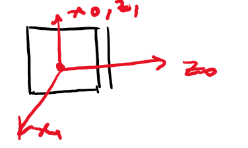
\includegraphics[scale = 0.5]{baseframe.png}\\[0.0 cm]	% University Logo
    \caption{Frame of Base}
  \end{subfigure}
\begin{subfigure}{.5\textwidth}
    \centering
    \textbf{EndEffector Frame}\par\medskip
    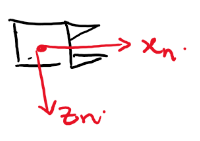
\includegraphics[scale = 0.5]{endeffecotrframe.png}\\[0.0 cm]	% University Logo
    \caption{Frame of EndEffector}
\end{subfigure}
\end{figure}

\textbf{Output}
Checking if the rotation matrix needed to transform the orientation of Base frame matches what we expect for EndEffector frame when robot 
has not been rotated.
Clearly this implies the
\begin{itemize}
  \item $x_n$ must point in the $z_0$ direction
  \item $z_n$ must point in the $y_0$ direction
  \item $y_n$ must point in the $x_0$ direction

\end{itemize}
\begin{figure}[H]
    \centering
    \textbf{Base Frame}\par\medskip
    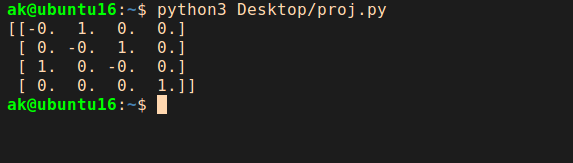
\includegraphics[scale = 0.8]{fkin.png}\\[0.0 cm]	% University Logo
    \caption{Frame of Base}
\end{figure}
Clearly this matches with the matrix obtained. Refer to \textbf{Appendix Section(Code for Forward Kinematics Test)}

\textbf{Inverse Kinematics Calculations} \\
 The verification of the inverse kinematics was done by manually inputing values and checking to see if the results 
match what was expected. This is not the ideal way to verify inverse kinematics calculations. Trying to calculations to vrep
was not trivial as it was difficult to track frames.

\newpage
\section{Results}
  The results of the simulation can be listed as follows:
  \begin{enumerate}
    \item Simulation of Forward and Inverse Kinematics - \textbf{Successful}
       \begin{enumerate}
         \item Robot is able to get to the metal sheet - \textbf{Successful}
         \item No singular configurations encounted from robot movements - \textbf{Successful}
         \item Robot is able to get to initial configuration - \textbf{Successful} 
         \item Robot is able to follow some specified path - \textbf{Successful}
       \end{enumerate}
     \item Simulation of Gripper - \textbf{partially successful}
         \begin{enumerate}
         \item Endeffector is placed at right location to weld metal sheets -\textbf{Successful}
         \item Endeffector pierces(close and open)metal sheet - \textbf{Not successful}
          \end{enumerate}
        \item Object dynamics  - \textbf{Not successful}
          \begin{enumerate}
            \item Metal sheet dynamics(force needed to pierce metal sheet) -\textbf{Not simulated}
            \item Included robot dynamics in simulation-\textbf{Not simulated}(Most of the dynamics of the welding robot was turned off )
          \end{enumerate}
        \item Mimicking Real World Scenario - \textbf{Partially successful}
          \begin{enumerate}
            \item Introducing probabilitic effects in the goods produced, that is defects in production -\textbf{Not simulated}
            \item Making the environment more elaborate -\textbf{Partially successful}(Simulation environment could be better)
          \end{enumerate}
        \item Testing and Verifying - \textbf{Partially successful}
          \begin{enumerate}
            \item Trying to match calculations with vrep calculations - \textbf{Partially successful} (In order to match the calculations outline above together
              vrep's, the frames utilized in vrep was hard to track. Need to learn how to use vrep and obtain such information )
          \end{enumerate}
  \end{enumerate}

\section{Conclusion and Future Work}
Based on the simulation, it could be noted that the endeffector is able to get to the desired location to weld the metalsheets.
However, the gripper(baxter gripper) used for the project is not appropriate for the application at hand. Future simulations would
rectify this by using a proper cad model for the endeffector(with a piering effect)  including necessary code and calcuations for
the visualization effect. Also, the dynamics of the robot model can be included to make the model more realistic.

\newpage
\section{Appendix}
This section has all the necessary codes used in calcuations and simulation
\subsection{Code for DH Table}
\lstinputlisting{../practice.m}

\subsection{Code for Jacobian}
\lstinputlisting{../p2.m}

\subsection{Simulation components used in Vrep}
Refer to \url{https://github.com/mesneym/RobotModelling} for the scene, code , and URDF files, used in vrep

\subsection{Code for Forward Kinematics Test}
\begin{lstlisting}
import numpy as np 

def transZ(n):
    a = np.identity(4)
    return a

def transX(n):
    a=np.identity(4)
    a[0,3]=n
    return a

def transY(n):
    a=np.identity(4)
    a[1,3]=n
    return a

def rotX(n):
    x=np.deg2rad(n)
    a=np.array([[1,0,0,0],
                [0,np.cos(x),-np.sin(x),0],
                [0,np.sin(x),np.cos(x),0 ],
                [0, 0,0,1]
               ])
    return a

def rotY(n):
    x=np.deg2rad(n)
    a=np.array([[np.cos(x),0,np.sin(x),0],
                [0,1,0,0],
                [-np.sin(x),0,np.cos(x),0 ],
                [0, 0,0,1]
               ])
    return a

def rotZ(n):
    x=np.deg2rad(n)
    a=np.array([[np.cos(x),-np.sin(x),0,0],
                [np.sin(x),np.cos(x),0,0],
                [0,0,1,0 ],
                [0,0,0,1]
               ])
    return a


def A_dh(theta,d,a,alpha):
   return  np.dot(rotZ(theta),
           np.dot(transZ(d),
           np.dot(transX(a),
           rotX(alpha))))



#Question Project
############################################################
##
#############################################################
q = [0, 0, 0, 0, 0]
l2 = l4  = 2
A1=A_dh(90,q[0],0,90)
A2=A_dh(q[1]+90,l2,0,90)
A3=A_dh(q[2]+90,0,0,90)
A4=A_dh(q[3]+90,l4,0,90)
A5=A_dh(q[4]+90,0,0,90)

T0_1 = A1
T0_2 = np.dot(T0_1,A2)
T0_3 = np.dot(T0_2,A3)
T0_4 = np.dot(T0_3,A4)
T0_5 = np.dot(T0_4,A5)

print(np.round(T0_5,3))
\end{lstlisting}


\section{References}
\bibliographystyle{plain}
\bibliography{biblist}

[1] \url{https://www.youtube.com/watch?v=N5AYZxsnDuM}

[2] \url{https://en.wikipedia.org/wiki/Arc_welding}

[3] \url{https://en.wikipedia.org/wiki/Robot_welding}

\end{document}
